\documentclass[a4paper,12pt]{report}

% ===========================
% Encodage et langue
% ===========================
\usepackage[utf8]{inputenc}
\usepackage[T1]{fontenc}
\usepackage[french]{babel}

% ===========================
% Mise en page
% ===========================
\usepackage{geometry}
\usepackage{setspace}
\usepackage{fancyhdr}

\usepackage{newtxtext,newtxmath}

% ===========================
% Couleurs et cadres
% ===========================
\usepackage{xcolor}
\usepackage{mdframed}
\usepackage{soul}

% ===========================
% Sommaire
% ===========================
\usepackage{tocloft}
\setcounter{tocdepth}{2}
\addto\captionsfrench{
    \renewcommand{\tablename}{Tableau}
    \renewcommand{\listfigurename}{Liste des figures}
    \renewcommand{\listtablename}{Liste des tableaux}
}

% ===========================
% Diagrammes
% ===========================
\usepackage{tikz}
\usetikzlibrary{arrows.meta,shapes,positioning, calc}

% ===========================
% Chapitres sans "Chapitre"
% ===========================
\usepackage{titlesec}
\titleformat{\chapter}
{\bfseries\LARGE} % style
{\thechapter.}               % numéro suivi d'un point
{1em}                        % espace entre numéro et titre
{}                            % code avant le titre
\setcounter{secnumdepth}{4}
\setcounter{tocdepth}{4}

\titleformat{\section}
{\bfseries\Large}
{\thesection}{1em}{}

\titleformat{\subsection}
{\bfseries\large}
{\thesubsection}{1em}{}

% ===========================
% Marges et interligne
% ===========================
\geometry{top=1.5cm, bottom=2cm, left=3.5cm, right=2.5cm}
\onehalfspacing

% ===========================
% Hyperliens
% ===========================
\usepackage{hyperref}
\hypersetup{
    colorlinks=true,
    linkcolor=blue,
    urlcolor=blue
}

% ===========================
% Entête simple pour le reste du document
% ===========================
\usepackage{fancyhdr}
\pagestyle{fancy}
\fancyhf{} % vide le header et footer
\fancyhead[C]{Conception d’une plateforme pédagogique de cybersécurité pour la simulation et la détection des cyberattaques dans une application web} % titre abrégé à gauche
\fancyfoot[R]{\thepage}
\renewcommand{\headrulewidth}{0.4pt} % ligne sous l'entête
\renewcommand{\footrulewidth}{0pt} % pas de ligne de pied de page

\fancypagestyle{plain}{
    \fancyhf{}
    \fancyfoot[R]{\thepage}
}

\usepackage{caption}
\usepackage{graphicx}
\usepackage{float}

\usepackage{url}

\usepackage{lettrine}

\usepackage{pdflscape}

\begin{document}
    
    % ===========================
    % PAGE DE GARDE
    % ===========================
    \begin{titlepage}
        
        \begin{tikzpicture}[remember picture, overlay]
            \draw[black, ultra thick] 
            ([xshift=1cm,yshift=-1cm]current page.north west) rectangle 
            ([xshift=-1cm,yshift=1cm]current page.south east);
        \end{tikzpicture}
        
        \begin{center}
            
            % ===== Logos =====
            
\includegraphics[width=3cm, height=2.5cm]{ben.png}\hfill
            
\includegraphics[width=3.5cm, height=2.5cm]{lcs.jpg}
            
            \vspace{0.8cm}
            
            % ===== République =====
            {\Large\bfseries RÉPUBLIQUE DU BÉNIN}\\
            {\small ********}
            
            \vspace{0.5cm}
            
            {\normalsize\bfseries MINISTÈRE DE L'ENSEIGNEMENT SUPÉRIEUR ET DE LA RECHERCHE SCIENTIFIQUE}\\
            {\small ********}   
            
            \vspace{0.5cm}         
            
            {\normalsize\bfseries DIRECTION GÉNÉRALE DE L'ENSEIGNEMENT SUPÉRIEUR}\\
            {\small ********}
            
            \vspace{0.5cm}
            
            {\large\bfseries INSTITUT UNIVERSITAIRE LES COURS SONOU}\\
            {\small ********}
            
            \vspace{0.5cm}
            
            {\large\bfseries MÉMOIRE DE FIN DE FORMATION EN LICENCE PROFESSIONNELLE}\\
            
            \vspace{0.6cm}
            
            % ===== Filière / spécialité =====
            \begin{minipage}{0.45\textwidth}
                \raggedright
                \textbf{Filière :} Informatique
            \end{minipage}
            \hfill
            \begin{minipage}{0.45\textwidth}
                \raggedleft
                \textbf{Spécialité :} Sécurité Informatique
            \end{minipage}
            
            \vspace{1cm}
            
            % ===== Thème =====
            % ===== Thème =====
            {\bfseries THÈME}
            
            \vspace{0.4cm}
            
            \begin{mdframed}[backgroundcolor=blue!20, roundcorner=5pt, innertopmargin=0.4cm, innerbottommargin=0.4cm]
                \centering
                \small\bfseries
                Conception d’une plateforme pédagogique de cybersécurité pour la simulation et la détection des cyberattaques dans une application web
            \end{mdframed}
            
            \vspace{1cm}
            
            % ===== Auteurs =====
            \begin{minipage}{0.45\textwidth}
                \centering
                \textbf{Réalisé par :}\\[0.2cm]
                Olivier FATOMBI\\
                Adolphe GUERE
            \end{minipage}
            \hfill
            \begin{minipage}{0.45\textwidth}
                \centering
                \textbf{Encadré par :}\\[0.2cm]
                \textbf{Maître de mémoire :}\\
                Dr Issifou IMOROU\\[0.3cm]
                \textbf{Maître de stage :}\\
                Mme DOVONOU Corine
            \end{minipage}
            
            \vfill
            
            {\bfseries Année universitaire : 2025 -- 2026}
            
        \end{center}
        
    \end{titlepage}
    
    \chapter*{AVERTISSEMENT}
    \addcontentsline{toc}{chapter}{AVERTISSEMENT}
    
    \begin{mdframed}[
        backgroundcolor=white,
        linecolor=black,
        linewidth=1pt,
        roundcorner=5pt,
        innertopmargin=10pt,
        innerbottommargin=10pt,
        innerleftmargin=10pt,
        innerrightmargin=10pt
        ]
        \centering
        L’Institut Universitaire Les Cours Sonou de Parakou n’entend donner ni approbation ni improbation aux idées émises dans ce mémoire. Celles-ci doivent être considérées comme propres à leurs auteurs.
        
    \end{mdframed}
    
    \chapter*{DÉDICACE 1}
    \addcontentsline{toc}{chapter}{DÉDICACE 1}
    
    \lettrine{A}{ mes chers parents FATOMBI Jacques et OWODINAN Solange, mes frère et sœur, ainsi qu’à KPAKPA Immaculée, pour leur soutien indéfectible tout au long de ce parcours.}
    
    \vspace{2cm}
    
    \begin{flushright}
        \large\bfseries{FATOMBI Olivier}
    \end{flushright}
    
    \chapter*{DÉDICACE 2}
    \addcontentsline{toc}{chapter}{DÉDICACE 2}
    
    \chapter*{REMERCIEMENTS}
    \addcontentsline{toc}{chapter}{REMERCIEMENTS}
    
    Ce mémoire est l’aboutissement de nombreuses recherches et d’un travail rigoureux et dévoué. Il n’aurait pu être réalisé sans les contributions précieuses de nombreuses personnes.
    
    Nous exprimons ainsi nos sincères remerciements à toutes celles et tous ceux qui, de près ou de loin, ont contribué à la réalisation de ce travail.
    
    Nos remerciements s’adressent tout particulièrement à :
    
    \begin{itemize}
        \item Dr IMOROU Issifou, notre maître de mémoire, enseignant à l’Institut Universitaire LES COURS SONOU de Parakou, pour les connaissances qu’il nous a transmises tout au long de notre formation, ainsi que pour sa disponibilité, ses conseils et son accompagnement ;
        
        \vspace{0.5cm}
        \item Madame DOVONOU Corine, responsable de l'équipe COSIT Bénin, pour ses orientations et conseils lors de la conception de nos projets ;
        
        \vspace{0.5cm}
        \item Toute l’équipe pédagogique et administrative de l’Institut Universitaire LES COURS SONOU de Parakou, pour leur encadrement et leur contribution à notre formation académique et professionnelle ;
        
        \vspace{0.5cm}
        \item Les honorables membres du jury, pour l’intérêt porté à notre travail et pour l’évaluation qu’ils en feront ;
        
        \vspace{0.5cm}
        \item Nos parents, nos frères et sœurs, pour leur soutien indéfectible, leurs encouragements et leur accompagnement tout au long de notre parcours ;
        
        \vspace{0.5cm}
        \item Nos camarades et amis de l’Institut Universitaire LES COURS SONOU de Parakou, en particulier ceux de la filière Sécurité des Système et Réseau Informatique ;
        
        \vspace{0.5cm}
        \item Toutes les personnes qui, de près ou de loin, ont contribué à la réalisation de ce mémoire.
    \end{itemize}
    
    \chapter*{LISTE DES SIGLES ET ABRÉVIATIONS}
    \addcontentsline{toc}{chapter}{LISTE DES SIGLES ET ABRÉVIATIONS}
    
    \begin{table}[H]
        \centering
        \begin{tabular}{p{4cm} p{10cm}}
            
            \textbf{OTP} & One-Time Password (mot de passe à usage unique) \\
            
            \textbf{XSS} & Cross-Site Scripting (attaque permettant d’injecter du code JavaScript malveillant dans une application web) \\
            
            \textbf{SQL} & Structured Query Language (langage de gestion des bases de données) \\
            
            \textbf{IDS} & Intrusion Detection System (système de détection d’intrusion) \\
            
            \textbf{IP} & Internet Protocol (adresse identifiant un équipement sur un réseau) \\
            
            \textbf{HTTP} & HyperText Transfer Protocol (protocole de communication web) \\
            
            \textbf{HTTPS} & HyperText Transfer Protocol Secure (version sécurisée du protocole HTTP) \\
            
            \textbf{RBAC} & Role-Based Access Control (contrôle d’accès basé sur les rôles) \\
            
            \textbf{CSRF} & Cross-Site Request Forgery (attaque visant à exécuter des actions à l’insu d’un utilisateur authentifié) \\
            
            \textbf{SOC} & Security Operations Center (centre de supervision de la sécurité) \\
            
        \end{tabular}
    \end{table}
    
    \newpage
    \addcontentsline{toc}{chapter}{LISTE DES TABLEAUX}
    \listoftables
    
    \newpage
    \addcontentsline{toc}{chapter}{LISTE DES FIGURES}
    \listoffigures
    
    % ===========================
    % RÉSUMÉ (FR)
    % ===========================
    \chapter*{RÉSUMÉ}
    \addcontentsline{toc}{chapter}{RÉSUMÉ} % ajoute au sommaire
    
    Ce mémoire porte sur la conception et le développement d’une plateforme pédagogique de cybersécurité permettant de simuler et de détecter des cyberattaques dans une application web.
    
    Dans un contexte où les systèmes d’information sont de plus en plus exposés aux menaces, il est essentiel de disposer d’outils permettant de comprendre et d’illustrer les mécanismes de sécurité de manière concrète.
    
    La solution proposée, nommée CyberGuard, intègre un système d’authentification renforcé, un module de journalisation des actions, un moteur de détection de certaines attaques (Brute Force, SQL Injection, XSS) ainsi qu’un tableau de bord de supervision.
    
    Le système repose sur un mini site métier servant de support de démonstration, permettant de générer des événements exploitables pour l’analyse.
    
    Les résultats obtenus montrent que la plateforme permet une meilleure compréhension des mécanismes de cybersécurité, tout en offrant une visualisation claire des incidents et des comportements suspects dans un environnement pédagogique contrôlé.
    
    \vspace{0.5cm}
    
    % ===========================
    % ABSTRACT (EN)
    % ===========================
    \chapter*{ABSTRACT}
    \addcontentsline{toc}{chapter}{ABSTRACT} % ajoute au sommaire
    
    This thesis focuses on the design and development of a pedagogical cybersecurity platform for simulating and detecting cyberattacks in a web application.
    
    In a context where information systems are increasingly exposed to threats, it is essential to provide tools that help understand and demonstrate security mechanisms in a practical way.
    
    The proposed solution, named CyberGuard, integrates strong authentication, user activity logging, a detection engine for common attacks (Brute Force, SQL Injection, XSS), and a monitoring dashboard.
    
    The system relies on a mini business application used as a demonstration environment to generate exploitable events for analysis.
    
    The results show that the platform improves the understanding of cybersecurity concepts while providing clear visualization of incidents and suspicious activities in a controlled environment.
    
    % ===========================
    % TABLE DES MATIÈRES
    % ===========================
    \clearpage
    \tableofcontents    
    \newpage
    
    
    % ===========================
    % CHAPITRE 1 : INTRODUCTION
    % ===========================
    \chapter{INTRODUCTION GÉNÉRALE}
    
    \section{Contexte et justificatif}
    
    Avec l’évolution rapide des technologies de l’information et de la communication, les systèmes informatiques sont devenus essentiels dans la gestion des organisations. Cependant, cette dépendance accrue aux technologies expose les systèmes à de nombreuses menaces, notamment les attaques informatiques.
    
    Les cyberattaques, telles que les attaques par force brute, les injections SQL ou encore les attaques XSS, constituent aujourd’hui des risques majeurs pour les applications web \cite{owasp}. Elles peuvent compromettre la confidentialité, l’intégrité et la disponibilité des données.
    
    \section{Problématique}
      
    Dans la plupart des organisations, les systèmes existants pour la surveillance et l'analyse des évènements de sécurité restent souvent peu fiables. Les conséquences peuvent inclure la perte de données sensibles, des interruptions de services ou la compromission des systèmes critiques. 
    
    Face à ces enjeux, il devient indispensable de mettre en place des mécanismes de sécurité efficaces permettant de détecter, d’analyser et de répondre aux incidents de sécurité. Toutefois, la compréhension de ces mécanismes reste complexe, notamment dans un cadre pédagogique. 
    
    C’est dans ce contexte que s’inscrit le projet de notre mémoire, qui vise à proposer une plateforme de démonstration permettant d’illustrer les principaux mécanismes de sécurité applicative.
    
    \section{Objectifs du mémoire}
    
    L'objectif général de ce mémoire est de concevoir et déployer une architecture sécurisée intégrant à la fois des mécanismes de prévention, de détection et de réaction face aux menaces.
    
    De manière spécifique, il s'agit de :
    
    \begin{itemize}
         \item sécuriser l’accès à une plateforme à l’aide d’un mécanisme d’authentification renforcé ;
        \item surveiller les activités des utilisateurs ;
        \item détecter certains types d’attaques informatiques ;
        \item générer des alertes en cas de comportement suspect ;
        \item offrir un environnement de démonstration pédagogique en cybersécurité.
    \end{itemize}
    
    \section{Méthodologie adoptée}
    
    La réalisation de ce projet s’est appuyée sur une démarche structurée en plusieurs étapes :
    
    \begin{itemize}
        \item l’analyse des besoins et la définition du cahier des charges ;
        \item la conception du système à l’aide de diagrammes UML ;
        \item le développement de l’application en utilisant le framework Laravel ;
        \item la mise en place des mécanismes de sécurité ;
        \item la phase de test et de validation.
    \end{itemize}
    
    Cette approche a permis de garantir la cohérence du système et de faciliter son développement.
    
    \section{Présentation de la structure d'accueil}
    
    \textbf{COSIT BÉNIN} est une entreprise spécialisée dans les prestations de services informatiques. Spécialisée dans la conception et le développement d'applications web et mobile, elle assure le déploiement des réseaux informatiques, la gestion et la création de base de données. Cette entreprise assure aussi un rôle de consultant auprès des entreprises et startups.
    
    \textbf{COSIT BÉNIN} représente une équipe de développeurs qualifiés, compétents et dynamiques, qui évoluent dans un environnement de travail moderne et propice à l'innovation. Ils accompagnent efficacement les entreprises dans la mise en place d'outils informatiques adaptés au contexte local et aux exigences du marché.
    
    \section{Structure du mémoire}
    
    Notre document est structuré en trois (03) parties : le premier chapitre est relatif à la revue de littérature et l'étude de l'existant. Le deuxième est dédié aux méthodes et choix techniques pour la conception du système. Enfin, le troisième et dernier chapitre est consacré à la présentation des résultats et à la discussion.
    
    \chapter{REVUE DE LITTÉRATURE}
    
    \section{Introduction}
    
    La sécurité des systèmes informatiques constitue aujourd’hui un enjeu majeur dans le développement des applications web. Face à l’augmentation des cyberattaques, il est essentiel de comprendre les différents mécanismes de protection, de détection et de réaction.
    
    Cette revue de littérature a pour objectif de présenter les concepts fondamentaux liés à la cybersécurité, ainsi que les principales techniques d’attaque et de défense utilisées dans les applications web.
    
    \section{Notions générales de cybersécurité}
    
    \subsection{Cybersécurité}
    
    La cybersécurité regroupe l’ensemble des techniques, outils et pratiques visant à protéger les systèmes informatiques contre les menaces et les attaques\cite{nist}.
    
    Elle repose principalement sur trois principes fondamentaux :
    
    \begin{itemize}
        \item \textbf{Confidentialité} : garantir que seules les personnes autorisées peuvent accéder aux informations ;
        \item \textbf{Intégrité} : assurer que les données ne sont pas modifiées de manière non autorisée ;
        \item \textbf{Disponibilité} : garantir que les systèmes et les données sont accessibles lorsque cela est nécessaire.
    \end{itemize}
    
    Ces principes constituent la base de toute stratégie de sécurité informatique.
    
    \subsection{Journaux d’audit}
    
    Les journaux d’audit enregistrent toutes les actions critiques réalisées sur le système. Ils permettent d’assurer la traçabilité et de vérifier la conformité des opérations, tout en facilitant la détection des comportements anormaux ou malveillants.
    
    Il faut s'assurer que les journaux d'audit peuvent faciliter les \textbf{enquêtes post-incident} en cas de compromission et garantir la \textbf{conformité} avec les normes et régulations existants (ISO 27001, GDPR) \cite{iso27001}.
    
    Il est aussi à noter que la sécurisation des logs (hashing, blockchain, stockage immuable) améliore la fiabilité de l'audit.
    
    \subsection{Authentification forte et 2FA}
    
    Pour sécuriser l’accès aux ressources sensibles, une authentification forte est nécessaire. L’utilisation de la double authentification (2FA) renforce la sécurité des systèmes \cite{nist} en exigeant un facteur supplémentaire, généralement un code temporaire envoyé par email, SMS ou généré par une application mobile. L'authentification peut être basée sur l'un des modèles de contrôle d'accès suivants :
    
    \begin{itemize}
        \item \textbf{RBAC (Role-Based Access Control)} : contrôle basé sur les rôles attribués aux utilisateurs.
        \item \textbf{ABAC (Attribute-Based Access Control)} : contrôle basé sur les attributs et le contexte (ex. localisation, heure, type d’appareil).
        \item \textbf{Hybride RBAC/ABAC} : combinaison des deux pour une sécurité renforcée.
    \end{itemize}
    
    \subsection{Gestion des logs et des alertes}
    
    La collecte et l’analyse des logs permettent de détecter rapidement des anomalies et de générer des alertes en cas d’événements suspects. Ces mécanismes sont essentiels pour la prévention proactive des cyberattaques et la gestion efficace des incidents de sécurité.
    
    \subsubsection{Collecte des événements de sécurité}
    
    La première étape de tout système de supervision est la collecte des évènements de sécurité. Nombreuses sont les solutions modernes telles que les \textbf{SIEM} (\textit{Security Information and Event Management}) \cite{ibm_siem} qui intègrent la collecte centralisée, le stockage sécurisé et l'utilisation des logs pour une analyse efficace. Elle repose sur :
    
    \begin{itemize}
        \item \textbf{Les journaux systèmes (logs)} : registres automatiques des activités sur les serveurs, applications et réseaux.
        \item \textbf{Les sondes réseau} : dispositifs qui capturent le trafic pour identifier des comportements anormaux.
        \item \textbf{Les agents logiciels} : programmes installés sur les machines pour remonter des événements vers une plateforme centralisée.
    \end{itemize}
    
    \subsubsection{Analyse et corrélation des événements}
    
    L’analyse des événements permet de détecter des anomalies et des incidents de sécurité. Elle peut être basée sur des signatures ou des comportements \cite{ids}. Les approches principales incluent :
    
    \begin{itemize}
        \item \textbf{Analyse signature-based} : détection basée sur des modèles connus d’attaques.
        \item \textbf{Analyse comportementale} : identification d’écarts par rapport au comportement normal des utilisateurs ou du système.
        \item \textbf{Corrélation multi-source} : croisement des événements provenant de plusieurs sources pour identifier des attaques complexes.
    \end{itemize}
    
    \section{Étude de l'existant}
    
    \subsection{Analyse de l'existant}
       
    Plusieurs solutions et frameworks sont largement utilisés pour la collecte et l’analyse des événements de sécurité. Ces outils offrent des fonctionnalités variées allant de la simple collecte de logs à l’analyse comportementale avancée et la génération d’alertes en temps réel.
    
    \subsubsection{IBM QRadar}
    
    IBM QRadar est une solution SIEM permettant de collecter, analyser et corréler les événements de sécurité \cite{qradar} afin de détecter les menaces en temps réel.
    
    Elle repose sur une architecture modulaire qui permet de collecter des logs, d'analyser des flux réseau et utilise un moteur de corrélation permettant d’identifier des comportements suspects. Les incidents détectés sont regroupés sous forme d’alertes appelées « offenses », facilitant leur analyse et leur priorisation.
    
    \begin{table}[H]
        \centering
        \begin{tabular}{|p{6cm}|p{6cm}|}
            \hline
            \textbf{Avantages} & \textbf{Limites} \\
            \hline
            Corrélation avancée des événements & Coût de licence élevé \\
            \hline
            Analyse en temps réel & Complexité de déploiement \\
            \hline
            Vision centralisée de la sécurité & Forte consommation de ressources \\
            \hline
            Capacité à traiter de grands volumes de données & Courbe d’apprentissage importante \\
            \hline
        \end{tabular}
        \caption{Avantages et inconvénients de IBM QRadar}
    \end{table}
    
    \subsubsection{ELK Stack}
    
    ELK Stack est une solution open-source de gestion et d’analyse de données composée de trois outils principaux : Elasticsearch, Logstash et Kibana \cite{elk}.
    
    Elle permet de collecter, stocker, analyser et visualiser des données issues de différentes sources, notamment les logs systèmes et applicatifs.
    
    Cependant, contrairement aux solutions SIEM complètes, ELK ne propose pas nativement un moteur de corrélation avancé ou une gestion intégrée des incidents, ce qui nécessite des configurations supplémentaires.
    
    \begin{table}[H]
        \centering
        \begin{tabular}{|p{6cm}|p{6cm}|}
            \hline
            \textbf{Avantages} & \textbf{Limites} \\
            \hline
            Solution open-source et gratuite & Absence de SIEM complet natif \\
            \hline
            Grande flexibilité et personnalisation & Configuration complexe \\
            \hline
            Puissante capacité de visualisation (Kibana) & Nécessite des outils complémentaires \\
            \hline
            Scalabilité élevée & Maintenance technique importante \\
            \hline
        \end{tabular}
        \caption{Avantages et inconvénients de ELK Stack}
    \end{table}
    
    Ces différentes solutions illustrent la diversité des approches en matière de supervision de la sécurité : certaines sont orientées SIEM global, d’autres analyse de logs ou détection d’intrusion.   
    
    Cependant, leur complexité et leur niveau d’exigence technique les rendent peu adaptées à un cadre pédagogique.
    
    Ces constats justifient le développement d’une solution sur mesure répondant aux besoins spécifiques d'un environnement contrôlé et intégrant des pratiques de sécurité modernes.
    
    \subsection{PROBLÉMATIQUE}
    
    \begin{center}
        \textit{Comment concevoir et implémenter une plateforme de cybersécurité permettant de simuler, détecter et visualiser des cyberattaques de manière simple, interactive et adaptée à un usage pédagogique ?}
    \end{center}
    
    \subsection{Intéret de la conception}
    
    La conception de notre système de détection s’inscrit dans une démarche visant à répondre aux limites identifiées dans les solutions existantes. Elle présente un intérêt à la fois pédagogique, technique et stratégique.
    
    D’une part, elle permet de proposer un environnement simplifié pour l’apprentissage des concepts de cybersécurité. D’autre part, elle constitue une base expérimentale pour la simulation et la visualisation des cyberattaques.
    
    \subsubsection{Analyse SWOT}
    
    L’analyse SWOT permet d’évaluer les forces, faiblesses, opportunités et menaces liées à un projet. Dans le cas de notre système, voici les résultats de l'analyse SWOT :
    
   \begin{table}[H]
       \centering
       \begin{tabular}{|p{6cm}|p{6cm}|}
           \hline
           \textbf{Forces} & \textbf{Faiblesses} \\
           \hline
           Solution pédagogique et accessible & Fonctionnalités limitées par rapport aux SIEM industriels \\
           \hline
           Architecture simple et modulaire & Données simulées (moins réalistes) \\
           \hline
           Facilité de déploiement & Absence de certaines fonctionnalités avancées \\
           \hline
           Visualisation claire des attaques & Scalabilité limitée \\
           \hline
       \end{tabular}
       
       \vspace{0.5cm}
       
       \begin{tabular}{|p{6cm}|p{6cm}|}
           \hline
           \textbf{Opportunités} & \textbf{Menaces} \\
           \hline
           Utilisation dans des contextes académiques & Concurrence des solutions open-source évoluées \\
           \hline
           Extension vers des fonctionnalités avancées & Évolution rapide des cybermenaces \\
           \hline
           Intégration avec d’autres outils de sécurité & Risque de mauvaise interprétation des simulations \\
           \hline
       \end{tabular}
       
       \caption{Analyse SWOT du système}
   \end{table}
   
   \subsubsection{Business Model Canvas (BMC)}
   
   Le Business Model Canvas permet de faire une liste des différents éléments qui oeuvrent à la création de valeur pour les utilisateurs. Nous l'utiliserons pour modéliser le fonctionnement économique de notre système nommé CyberGuard.
   
   \paragraph{Proposition de valeur :}
   
   CyberGuard est un environnement sécurisé, fiable et centralisé, permettant de prévenir les accès non autorisés et de détecter les comportements suspects. Il offre donc une plateforme pédagogique de simulation et de détection des cyberattaques.
   
   \paragraph{Segments de clients :}
   
   CyberGuard s'adresse principalement à toute organisation qui souhaite sécuriser leur système d'information interne. Il propose une solution intégrée combinant gestion des données de l'entreprise et mécanismes avancés de cybersécurité, notamment le contrôle d'accès multi-acteurs, la traçabilité des actions et la détection d'anomalies.
   
   \paragraph{Activités clés :}
   
   Les activités clés concernent les activités que couvrent le système. Ils comprennent le développement logiciel, la maintenance et les mises à jour, l'analyse des logs de sécurité, la détection d'anomalies, la gestion des utilisateurs et accès, la surveillance du système.
   
   \paragraph{Ressources clés :}
   
   Nos ressources essentielles sont constituées :
   
   \begin{itemize}
       \item Une équipe technique chargée de la conception, du développement et la sécurisation du système.
       \item Des données simulées (fictives) représentant les utilisateurs et leurs différents modules respectifs, utilisées pour les tests et la démonstration des fonctionnalités.
       \item Un environnement et une infrastructure serveur.
       \item Un hébergement local temporaire permettant de tester le système et le rendre accessible pour la phase de démonstration.
       \item Les outils de collaboration (GitHub) pour le suivi de l'évolution du système et la coordination du binôme.
   \end{itemize}
    
   \section{Conclusion}
    
    Ce chapitre a permis d'explorer les principaux concepts et travaux relatifs au contrôle d'accès et aux mécanismes de traçabilité dans les systèmes d'information. L'analyse des solutions existantes a mis en évidence leurs avantages, notamment en termes de digitalisation des processus et d'amélioration du suivi des activités. Toutefois, ces systèmes présentent encore des limites, en particulier sur le plan de la sécurité, du contrôle d'accès multi-acteurs et de la détection proactive des comportements suspects.
    
    Ces insuffisances justifient la nécessité de concevoir une solution plus avancée intégrant des mécanismes de sécurité renforcés et une analyse intelligente des activités. C'est dans cette optique que s'inscrit la plateforme \textbf{CyberGuard}, proposé dans ce mémoire.
    
    % ===========================
    \chapter{ARCHITECTURE TECHNIQUE}
    % ===========================
    
    \section{Introduction}
    
    Face à l'évolution rapide des cybermenaces, les organisations doivent disposer d'outils capables de surveiller en continu leurs infrastructures informatiques. L'absence de mécanismes de détection efficaces peut entraîner des pertes financières, des violations de données et des interruptions de service.
    
    La mise en place d'un système d'analyse des évènements de sécurité permet d'améliorer la visibilité sur les activités du système d'information et de renforcer la posture de sécurité globale.
    
    \section{Cahier des charges}
    
    Nous allons définir les fonctionnalités attendues ainsi que les contraintes techniques du système.
    
    \subsection{Présentation du thème}
    
    Notre projet consiste en la conception et le développement d’une plateforme web pédagogique de cybersécurité intégrant des mécanismes de détection et de simulation des cyberattaques.
    
    L’objectif est de proposer un système permettant d’illustrer les principaux concepts de sécurité applicative à travers une application web intégrant un mini site métier servant de support de démonstration.
    
    Le système permet de surveiller les actions des utilisateurs, de détecter certains comportements malveillants et de générer des alertes, dans un environnement contrôlé et adapté à un usage pédagogique.
    
    \subsection{Objectifs du projet}
    
    \subsubsection{Objectif général}
    
    Concevoir et développer une plateforme web sécurisée permettant de simuler et de détecter des cyberattaques dans un environnement pédagogique.
    
    \subsubsection{Objectifs spécifiques}  
    
    Ce système doit être capable :
    \begin{itemize}
        \item Sécuriser l'accès à une application web,
        \item Surveiller les activités utilisateurs,
        \item Détecter des comportements malveillants,
        \item Générer des alertes exploitables,
        \item Assister l'analyse des incidents de sécurité.
    \end{itemize}
    
    Ce positionnement permet de combiner \textbf{développement web et cybersécurité} dans une seule solution cohérente.
    
    \subsection{Fonctionnalités principales}
    
    CyberGuard est structuré autour des fonctionnalités suivantes :
    
    \begin{itemize}
        \item Authentification sécurisée avec OTP,
        \item Gestion d'un mini site métier (usagers, services, messages),
        \item Journalisation des actions utilisateurs,
        \item Détection d'attaques (Brute Force, SQL Injection, XSS),
        \item Tableau de bord de supervision,
        \item Simulation d'attaques pour démonstration.
    \end{itemize}
    
    Le mini site métier joue un rôle central en servant de \textbf{surface applicative de test et de démonstration}.
    
    \subsection{Contraintes du projet}
    
    Les contraintes prises en compte sont :
    
    \begin{itemize}
        \item Simplicité d'utilisation pour la démonstration,
        \item Cohérence pédagogique pour la soutenance,
        \item Limitation volontaire du périmètre (3 types d'attaques),
        \item Compatibilité avec un environnement local (HTTP),
        \item Temps de développement limité.
    \end{itemize}
    
    \section{Analyse des besoins}
    
    \subsection{Exigences fonctionnelles}
   
    \begin{itemize}
        \item Permettre à un utilisateur de se connecter de manière sécurisée,
        \item Gérer des données métiers simples,
        \item Enregistrer toutes les actions importantes,
        \item Détecter automatiquement certaines attaques,
        \item Visualiser les alertes et incidents,
        \item Simuler des scénarios d'attaque.
    \end{itemize}
    
    \subsection{Exigences non fonctionnelles}
    
    Les besoins non fonctionnels concernent principalement :
    
    \begin{itemize}
        \item \textbf{Sécurité} : protection des accès et des données,
        \item \textbf{Performance} : temps de réponse acceptable,
        \item \textbf{Maintenabilité} : code structuré et modulaire,
        \item \textbf{Lisibilité} : interface simple pour la démonstration,
        \item \textbf{Fiabilité} : fonctionnement stable lors de la soutenance.
    \end{itemize}
    
    \section{Choix techniques}
    
    \subsection{Technologies utilisées}
    
    Le système a été développé avec les technologies suivantes :
    
    \begin{itemize}
        \item \textbf{Backend} : PHP 8.2 avec Laravel 12
        \item \textbf{Frontend} : Blade + Tailwind CSS + Alpine.js
        \item \textbf{Base de données} : SQLite (développement), MySQL (production)
        \item \textbf{Outils} : Vite, Composer, npm
    \end{itemize}
    
    Nous avons choisi d'utiliser Laravel en raison de sa structure MVC claire, ses outils intégrés de sécurité, sa rapidité de développement.
    
    \subsection{Architecture système}
        
    CyberGuard a été conçu suivant une architecture modulaire basée sur l'utilisation des controllers, services, models, middleware et views.
    
    \begin{itemize}
        \item \textbf{Controllers} : permettent d'assurer la gestion des requêtes,
        \item \textbf{Services} : servent à appliquer les logiques métiers relatifs aux fonctionnalités,
        \item \textbf{Models} : permettent l'accès au données,
        \item \textbf{Middleware} : assure la sécurité et le contrôle,
        \item \textbf{Views} : servent l'interface utilisateur.
    \end{itemize}
    
     Cette séparation améliore la maintenabilité et la clarté du code.
    
    \subsection{Organisation fonctionnelle}
    
    Le système est organisé en cing (05) modules principaux qui sont : \textbf{authentification sécurisée}, \textbf{mini site métier}, \textbf{moteur de détection}, \textbf{supervision} (dashboard, alertes), \textbf{module de simulation}. Cette organisation assure une meilleure compréhension et une démonstration fluide.
    
    \section{Aspects de sécurité}
    
    La sécurité est un aspect central dans la conception de tout système, dans le but de protéger d'une part la nature sensible des données manipulées et d'autre part les fonctionnalités liées à la détection d'attaques. Cette section présente ainsi les risques de sécurité identifiés ainsi que les principales mesures de sécurité adoptées pour y faire face.
    
    
    \subsection{Risques de sécurité}
    
    Dans le cadre de la conception du système CyberGuard, nombreuses sont les risques de sécurité qui ont été identifiés. Ces risques correspondent aux menaces informatiques les plus courantes dans les applications web.
    
    \subsubsection{Attaque par force brute (Brute Force)}
    
    L'attaquant cible principalement les interfaces d'authentification, et teste un grand nombre de combinaisons de mots de passe afin d'accéder à un compte utilisateur. Il peut automatiser les tentatives et compromettre un compte, surtout avec des mots de passe faibles et réutilisés \cite{owasp}.
    
    \subsubsection{Injection SQL}
    
    Cette attaque consiste à insérer du code SQL malveillant dans les champs de saisie d'une application afin de manipuler les requêtes exécutées sur la base de données. Le but pour un attaquant est de créer une faille dans les requêtes qui ne sont pas correctement sécurisées, lui donnant accès aux données sensibles, voire lui permettre de modifier, supprimer des informations ou de contourner le système d'authentification \cite{owasp}.
    
    \subsubsection{Cross-Site Scripting (XSS)}
    
    L'attaque XSS consiste à voler des cookies de session, la redirection vers des sites frauduleux ou la modification de l'interface affichée, grâce à des injections de code JavaScript malveillant dans une application web. Ainsi pour un utilisateur de cette application web, le code malveillant sera exécuté dans le navigateur, permettant de détecter les manques de validation ou d'échappement des données affichées afin de les exploiter \cite{owasp}.
    
    \subsubsection{Absence de traçabilité des actions}
    
    Il est difficile d'identifier l'origine d'un incident de sécurité ou de comprendre les action effectuées par un utilisateur, sans un mécanisme de journalisation des actions. Cette absence de logs limite donc fortement la capacité d'analyse et de réaction face à une attaque.
    
    \subsection{Mesures de sécurité}
    
    Afin d'éliminer ces différents risques de sécurité, nous avons intégré plusieurs mécanismes dans le système pour renforcer la sécurité globale de l'application.
    
    \subsubsection{Limitation de débit (rate limiting)}
    
    Elle a été mise en place sur les points sensibles de système d'authentification et vise à protéger contre les attaques par force brute. Les tentatives sont temporairement bloquées, après un certain nombre d'échecs, et permettent donc de ralentir de manière considérable les attaques automatisées et de protéger les comptes utilisateurs.
    
    \subsubsection{Renforcement du mécanisme d'authentification}
    
    L'authentification repose sur un processus en deux (02) étapes : la \textbf{vérification de l'email et du mot de passe} et la \textbf{validation d'un code OTP envoyé par email}. Un état intermédiaire est utilisé pour garantir que chaque étape est correctement respectée avant l'accès au système, cela empêche les contournements du processus d'authentification.    
    
    \subsubsection{Requêtes SQL paramétrées}
    
    Ces requêtes sont utilisées afin d'éviter l'injection du code SQL malveillant. Toutes les entrées utilisateur sont validées et traitées de manière sécurisée, ce qui empêche l'exécution de requêtes non autorisées sur la base de données.
    
    \subsubsection{Protection contre les attaques XSS}
    
    Les données affichées dans l'interface sont systématiquement échappées afin d'éviter l'exécution de scripts malveillants dans le navigateur. De plus, une validation des entrées utilisateur est effectuée pour détecter et bloquer les contenus suspects. Cela permet de réduire fortement les risques d'injection de code côté client.
    
    \subsubsection{Sécurisation des sessions}
    
    Le système met en place une gestion sécurisée des sessions à travers : l’utilisation de cookies httpOnly pour empêcher l’accès via JavaScript, l’attribut sameSite pour limiter les attaques inter-sites, une vérification de la validité des sessions côté serveur.
    
    Ces mesures permettent de réduire les risques de vol ou de détournement de session.
    
    \subsubsection{Gestion des rôles et des permissions}
    
    Un système de contrôle d’accès basé sur les rôles (RBAC) a été mis en place afin de limiter les actions accessibles à chaque type d’utilisateur. Chaque requête vers une ressource protégée est vérifiée afin de s’assurer que l’utilisateur dispose des autorisations nécessaires, ce qui réduit les risques d’accès non autorisé.
    
    \subsubsection{Mise en place d'un système de journalisation}
    
    Toutes les actions importantes (connexions, modifications, incidents) sont enregistrées dans des journaux. Cette traçabilité permet d’analyser les comportements suspects, de reconstituer les événements en cas d’incident et d’améliorer la supervision globale du système.
    
    \subsubsection{Détection et réaction aux comportements malveillants}
    
    Le système intègre un moteur de détection centré sur trois types d’attaques : Brute Force; Injection SQL; XSS.
    
    Lorsqu’un comportement suspect est détecté, une alerte est générée et peut entraîner des actions automatiques, comme le blocage d’une adresse IP. Cela permet une réaction rapide face aux menaces identifiées.\\
    
    L’ensemble de ces mécanismes permet de mettre en place une approche de sécurité multicouche, combinant prévention, détection et réaction. Dans la section suivante, nous présentons la modélisation du système, qui permet de visualiser clairement son fonctionnement et son architecture.
     
    \section{Modélisation}
    
    \subsection{Présentation et classification des acteurs}
    
    Dans le cadre de la modélisation du système \textbf{CyberGuard}, il est essentiel d’identifier les différents acteurs interagissant avec l’application. Un acteur représente toute entité externe (humaine ou non) capable d’interagir avec le système.
    
    Les principaux acteurs identifiés sont les suivants :
    
    \begin{itemize}
        \item Administrateur Système
        \item Attaquant
        \item Utilisateur du mini site métier
    \end{itemize}
    
    \subsubsection{Administrateur Système}
    
    L’administrateur système constitue l’acteur principal de la plateforme. Il est responsable de la gestion globale du système, aussi bien sur le plan technique que fonctionnel.
    
    Ses principales responsabilités incluent :
    
    \begin{itemize}
        \item la gestion des utilisateurs et des accès ;
        \item la supervision du tableau de bord de sécurité ;
        \item la consultation et l’analyse des alertes générées ;
        \item le traitement des incidents (investigation, blocage d’adresses IP, résolution) ;
        \item le suivi du bon fonctionnement du système.
    \end{itemize}
    
    Il joue également un rôle clé dans la démonstration du système en interprétant les résultats fournis par le moteur de détection.
    
    \subsubsection{Attaquant}
    
    L’attaquant est un acteur particulier introduit dans le cadre des simulations de cybersécurité. Il ne représente pas un utilisateur réel du système, mais une entité permettant de tester les mécanismes de détection.
    
    Son rôle consiste à :
    
    \begin{itemize}
        \item simuler des tentatives d’intrusion ;
        \item injecter des données malveillantes (SQL, scripts) ;
        \item effectuer des tentatives de connexion répétées (force brute) ;
        \item interagir avec les mécanismes de détection et les éventuels honeypots.
    \end{itemize}
    
    Cet acteur permet de valider le comportement du système face à des menaces réelles dans un environnement contrôlé.
    
    \subsubsection{Utilisateur du mini site métier}
    
    L’utilisateur du mini site métier représente un utilisateur légitime de l’application. Il interagit avec les fonctionnalités métiers qui servent de support à la démonstration du système.
    
    Cet acteur peut être subdivisé en plusieurs profils :
    
    \begin{itemize}
        \item \textbf{Utilisateur standard} : consulte et manipule les données du mini site (usagers, services, messages) ;
        \item \textbf{Gestionnaire} : effectue des opérations de création, modification ou suppression de données ;
        \item \textbf{Utilisateur observé} : ses actions sont journalisées et analysées par le système de détection.
    \end{itemize}
    
    Les interactions de cet acteur permettent de générer des événements exploitables par le système CyberGuard, notamment pour la détection d’activités suspectes et la production d’alertes.
    
    \subsection{Modélisation dynamique du système}
    
    \subsubsection{Diagramme de cas d'utilisation}
    
    \begin{figure}[H]
        \centering
        \includegraphics[width=\textwidth]{images/Cyberguard.png}
        \caption{Diagramme de cas d'utilisation global - CyberGuard}
    \end{figure}
    
    \begin{figure}[H]
        \centering
        \includegraphics[width=\textwidth]{images/CyberguardAdminSysteme.png}
        \caption{Diagramme de cas d'utilisation côté administrateur - CyberGuard}
    \end{figure}
    
    \begin{figure}[H]
        \centering
        \includegraphics[width=\textwidth]{images/CyberguardMiniSite.png}
        \caption{Diagramme de cas d'utilisation côté utilisateur - CyberGuard}
    \end{figure}
    
    \subsubsection{Description textuelle du cas d’utilisation « Se connecter »}
    
    \textbf{Titre :} Se connecter
       
    \textbf{Résumé :}  
    Ce cas d’utilisation permet à un utilisateur d’accéder au système CyberGuard via un processus d’authentification sécurisé basé sur un email, un mot de passe et un code OTP.
     
    \textbf{Précondition :}  
    Le système est accessible et l’utilisateur possède un compte valide.  
    
    \textbf{Acteurs :}  
    Utilisateur (Administrateur ou Utilisateur du mini site métier)
       
    \textbf{Date de création :} 05/03/2026
    
    \textbf{Version :} 1.0
    
    \textbf{Responsable :} FATOMBI Olivier et GUERE Adolphe
    
    \textbf{Description des scénarios :}
    
    \textbf{Scénario nominal}
    
    \begin{table}[H]
        \centering
        \begin{tabular}{|p{6cm}|p{6cm}|}
            \hline
            \textbf{Acteurs} & \textbf{Système} \\
            \hline
            1. L’utilisateur accède à la page de connexion & \\
            2. Il saisit son email et son mot de passe & \\
            \hline
            & 3. Le système vérifie les identifiants \\
            & 4. Le système génère et envoie un code OTP \\
            \hline
            5. L’utilisateur saisit le code OTP & \\
            \hline
            & 6. Le système vérifie le code OTP \\
            & 7. Le système crée une session sécurisée \\
            & 8. Le système redirige l’utilisateur vers le dashboard \\
            \hline
        \end{tabular}
        \caption{Scénario nominal du cas d’utilisation « Se connecter » - CyberGuard}
    \end{table}
    
    \textbf{Scénario alternatif}
    
    \textbf{A1 : Identifiants incorrects}
    
    Le système affiche un message d’erreur et l’utilisateur doit ressaisir ses informations.
    
    \textbf{A2 : Code OTP invalide ou expiré}
     
    Le système refuse l’accès et propose le renvoi d’un nouveau code OTP.
    
    \textbf{Postcondition :}  
    L’utilisateur est authentifié et accède au système.
    
    \textbf{Remarques :}  
    Ce mécanisme repose sur une authentification à deux facteurs renforçant la sécurité du système.
    
    \subsubsection{Description textuelle du cas d’utilisation « Gérer un incident »}
    
    \textbf{Titre :} Gérer un incident  
    
    \textbf{Résumé :}  
    Ce cas d’utilisation permet à un administrateur de consulter, analyser et traiter un incident de sécurité détecté par le système.
    
    \textbf{Précondition :}  
    L’utilisateur est authentifié et des incidents existent dans le système.
    
    \textbf{Acteurs :}  
    Administrateur
    
    \textbf{Date de création :} 20/03/2026 
     
    \textbf{Version :} 1.0  
    
    \textbf{Responsable :} FATOMBI Olivier et GUERE Adolphe
    
    \textbf{Description des scénarios :}
    
    \textbf{Scénario nominal}
    
    \begin{table}[H]
        \centering
        \begin{tabular}{|p{6cm}|p{6cm}|}
            \hline
            \textbf{Acteurs} & \textbf{Système} \\
            \hline
            1. L’utilisateur accède à la liste des incidents & \\
            2. Il sélectionne un incident & \\
            \hline
            & 3. Le système affiche les détails de l’incident \\
            \hline
            4. L’utilisateur analyse les informations & \\
            5. L’utilisateur modifie le statut (investigating, blocked, resolved) & \\
            \hline
            & 6. Le système enregistre la mise à jour \\
            & 7. Le système met à jour les informations dans le dashboard \\
            \hline
        \end{tabular}
        \caption{Scénario nominal du cas d’utilisation « Gérer un incident » - CyberGuard}
    \end{table}
    
    \textbf{Scénario alternatif}
    
    \textbf{A1 : Incident inexistant}
      
    Le système affiche un message indiquant que l’incident est introuvable.
    
    \textbf{Postcondition :}  
    L’incident est traité et son statut est mis à jour.
    
    \textbf{Remarques :}  
    Ce cas d’utilisation est essentiel pour la supervision et la réponse aux menaces.
    
    \subsubsection{Description textuelle du cas d’utilisation « Utiliser le mini site métier »}
    
    \textbf{Titre :} Utiliser le mini site métier  
    
    \textbf{Résumé :}  
    Ce cas d’utilisation permet à un utilisateur d’interagir avec les fonctionnalités du mini site métier afin de consulter et manipuler des données (usagers, services, messages).
    
    \textbf{Précondition :}  
    L’utilisateur est authentifié.
    
    \textbf{Acteurs :}  
    Utilisateur du système
    
    \textbf{Date de création :} 21/04/2026  
    
    \textbf{Version :} 1.0  
    
    \textbf{Responsable :} FATOMBI Olivier et GUERE Adolphe
    
    \textbf{Description des scénarios :}
    
    \textbf{Scénario nominal}
    
    \begin{table}[H]
        \centering
        \begin{tabular}{|p{6cm}|p{6cm}|}
            \hline
            \textbf{Acteurs} & \textbf{Système} \\
            \hline
            1. L’utilisateur accède au mini site métier & \\
            2. Il consulte les données disponibles & \\
            3. Il effectue une action (ajout, modification ou suppression) & \\
            \hline
            & 4. Le système enregistre l’action \\
            & 5. Le système déclenche un événement de journalisation \\
            & 6. Le système analyse l’action pour détecter un comportement suspect \\
            \hline
        \end{tabular}
        \caption{Scénario nominal du cas d’utilisation « Utiliser le mini site métier » - CyberGuard}
    \end{table}
    
    \textbf{Scénario alternatif}
    
    \textbf{A1 : Données invalides}
      
    Le système affiche un message d’erreur et demande une correction.
    
    \textbf{A2 : Comportement suspect détecté}  
    
    Le système génère une alerte et enregistre un incident.
    
    \textbf{Postcondition :}  
    Les données sont mises à jour et les actions sont journalisées.
    
    \textbf{Remarques :}  
    Le mini site métier sert de support de démonstration pour le moteur de détection du système.
    
    \subsubsection{Diagramme de classes}
    
    Le diagramme de classes représente la structure statique du système CyberGuard. Il permet de modéliser les différentes entités du système ainsi que les relations qui existent entre elles.
    
    \begin{figure}[H]
        \centering
        \includegraphics[width=\textwidth]{images/CyberguardClassDiagram.png}
        \caption{Diagramme de classes - CyberGuard}
    \end{figure}
    
    \begin{figure}[H]
        \centering
        \includegraphics[width=\textwidth]{images/CyberguardClassDiagramG.png}
        \caption{Diagramme de classes - CyberGuard}
    \end{figure}
    
    \begin{figure}[H]
        \centering
        \includegraphics[width=\textwidth]{images/CyberguardClassDiagramD.png}
        \caption{Diagramme de classes - CyberGuard}
    \end{figure}
    
    \subsubsection{Diagramme de déploiement}
    
    \begin{figure}[H]
        \centering
        
\includegraphics[width=0.8\textwidth]{images/CyberGuardDeployment.png}
        \caption{Diagramme de déploiement - CyberGuard}
    \end{figure}
    
    \subsubsection{Diagramme de séquence}
    
    \begin{figure}[H]
        \centering
        \includegraphics[width=0.8\textwidth]{images/CyberguardSequenceAuthentification.png}
        \caption{Séquence d'authentification - Email / mot de passe / OTP / session sécurisée - CyberGuard}
    \end{figure}
    
    \begin{figure}[H]
        \centering
        \includegraphics[width=0.8\textwidth]{images/CyberguardSequenceGenerale.png}
        \caption{Séquence generale - mini site éetier, audit, détection, alerte et analyse SOC - CyberGuard}
    \end{figure}
    
    \begin{figure}[H]
        \centering
        \includegraphics[width=0.8\textwidth]{images/CyberguardSequenceControleAcces.png}
        \caption{Séquence de controle d'accès - IP, session, role et audit - CyberGuard}
    \end{figure}
    
    \section{Conclusion}
    
    Dans ce chapitre, nous avons présenté les méthodes et choix techniques adoptés pour la conception du système CyberGuard. L’analyse des besoins, les choix technologiques, les aspects de sécurité ainsi que la modélisation UML ont permis de définir une architecture claire, cohérente et adaptée aux objectifs du projet.
    
    Ces éléments constituent une base solide pour la réalisation du système, qui sera abordée dans le chapitre suivant.
    
    \chapter{RÉSULTATS OBTENUS}
    
    \section{Introduction}
    
    Ce chapitre présente les résultats obtenus à l’issue de la conception et du développement du système CyberGuard. Il met en évidence les fonctionnalités réalisées, les tests effectués ainsi que les performances globales du système.
    
    L’objectif est de démontrer que les choix techniques et méthodologiques adoptés ont permis de concevoir une application fonctionnelle, cohérente et conforme aux besoins définis dans le cahier des charges.
    
    \section{Présentation générale du système réalisé}
    
    Le système CyberGuard développé est une application web de cybersécurité permettant de sécuriser l’accès à une plateforme, de surveiller les activités utilisateurs et de détecter certaines attaques informatiques.
    
    Il repose sur une architecture modulaire intégrant plusieurs composants, notamment un système d’authentification renforcé, un mini site métier servant de support de démonstration, un moteur de détection d’attaques et un tableau de bord de supervision.
    
    Le système permet ainsi de combiner des fonctionnalités de prévention, de détection et de réaction face aux menaces de sécurité.
    
    \section{Fonctionnalités implémentées}
    
    Les principales fonctionnalités implémentées dans le système sont les suivantes :
    
    \begin{itemize}
        \item Authentification sécurisée basée sur un mot de passe et un code OTP ;
        \item Gestion des sessions sécurisées ;
        \item Mini site métier permettant la gestion des données (usagers, services, messages) ;
        \item Journalisation des actions utilisateurs ;
        \item Détection d’attaques (Brute Force, SQL Injection, XSS) ;
        \item Génération d’alertes en cas de comportement suspect ;
        \item Tableau de bord de supervision ;
        \item Gestion des incidents de sécurité ;
        \item Simulation d’attaques pour démonstration.
    \end{itemize}
    
    Ces fonctionnalités permettent de répondre aux principaux besoins identifiés lors de l’analyse du système.
    
    \section{Résultats des tests et validation}
    
    Plusieurs tests ont été réalisés afin de vérifier le bon fonctionnement du système et valider les fonctionnalités implémentées.
    
    Les tests d’authentification ont permis de confirmer le bon déroulement du processus de connexion avec OTP, ainsi que la gestion correcte des erreurs en cas d’identifiants ou de code invalide.
    
    Les tests de détection ont montré que le système est capable d’identifier les comportements suspects liés aux attaques par force brute, aux injections SQL et aux attaques XSS. Dans chaque cas, une alerte est générée et un incident peut être créé.
    
    Les tests du mini site métier ont permis de valider la création, la modification et la suppression des données, ainsi que leur journalisation.
    
    De manière générale, les résultats obtenus confirment la stabilité et la cohérence du système.
    
    \section{Illustration du système}
    
    Afin de mieux visualiser les résultats obtenus, plusieurs interfaces du système ont été réalisées, notamment :
    
    \begin{itemize}
        \item la page de connexion avec authentification OTP ;
        \item le tableau de bord de supervision ;
        \item le centre d’alertes ;
        \item la gestion des incidents ;
        \item le mini site métier.
    \end{itemize}
    
    Ces interfaces permettent de démontrer le fonctionnement réel du système et facilitent sa compréhension lors de la présentation.
    
    \subsection{Page de connexion avec authentification OTP}
    
    \begin{figure}[H]
        \centering
        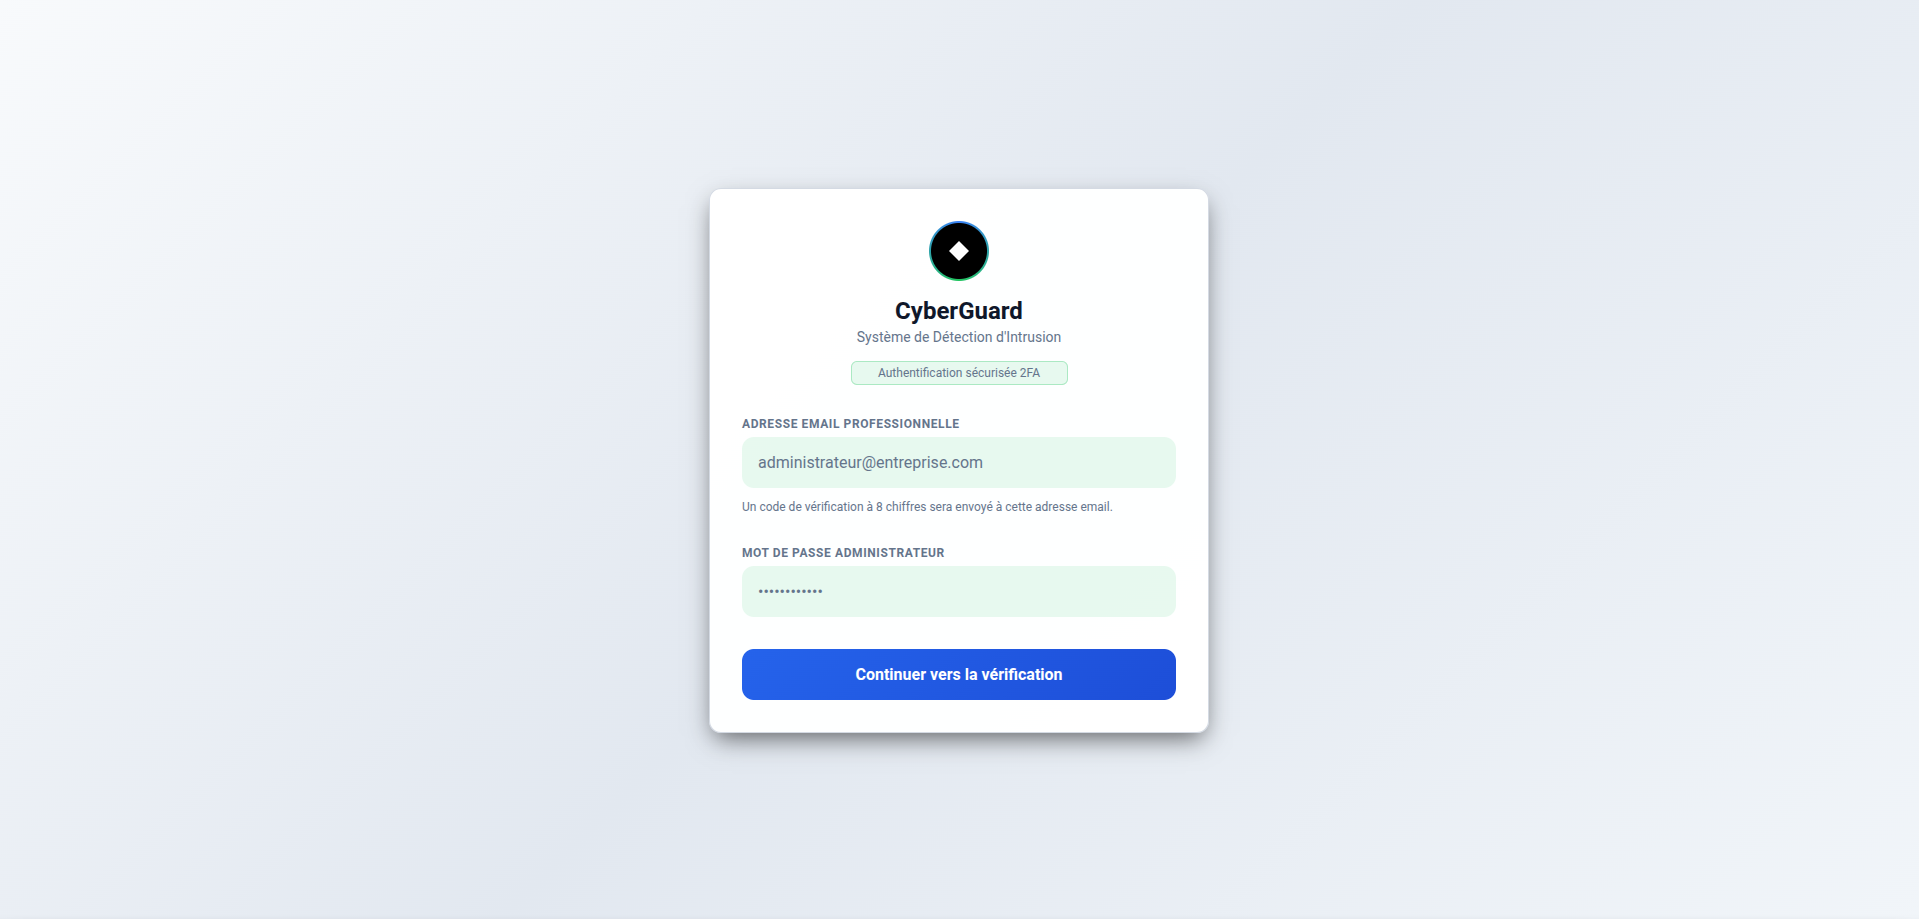
\includegraphics[width=0.8\textwidth]{images/vue-login.png}
        \caption{Vue connexion email + mot de passe - CyberGuard}
    \end{figure}
    
    \begin{figure}[H]
        \centering
        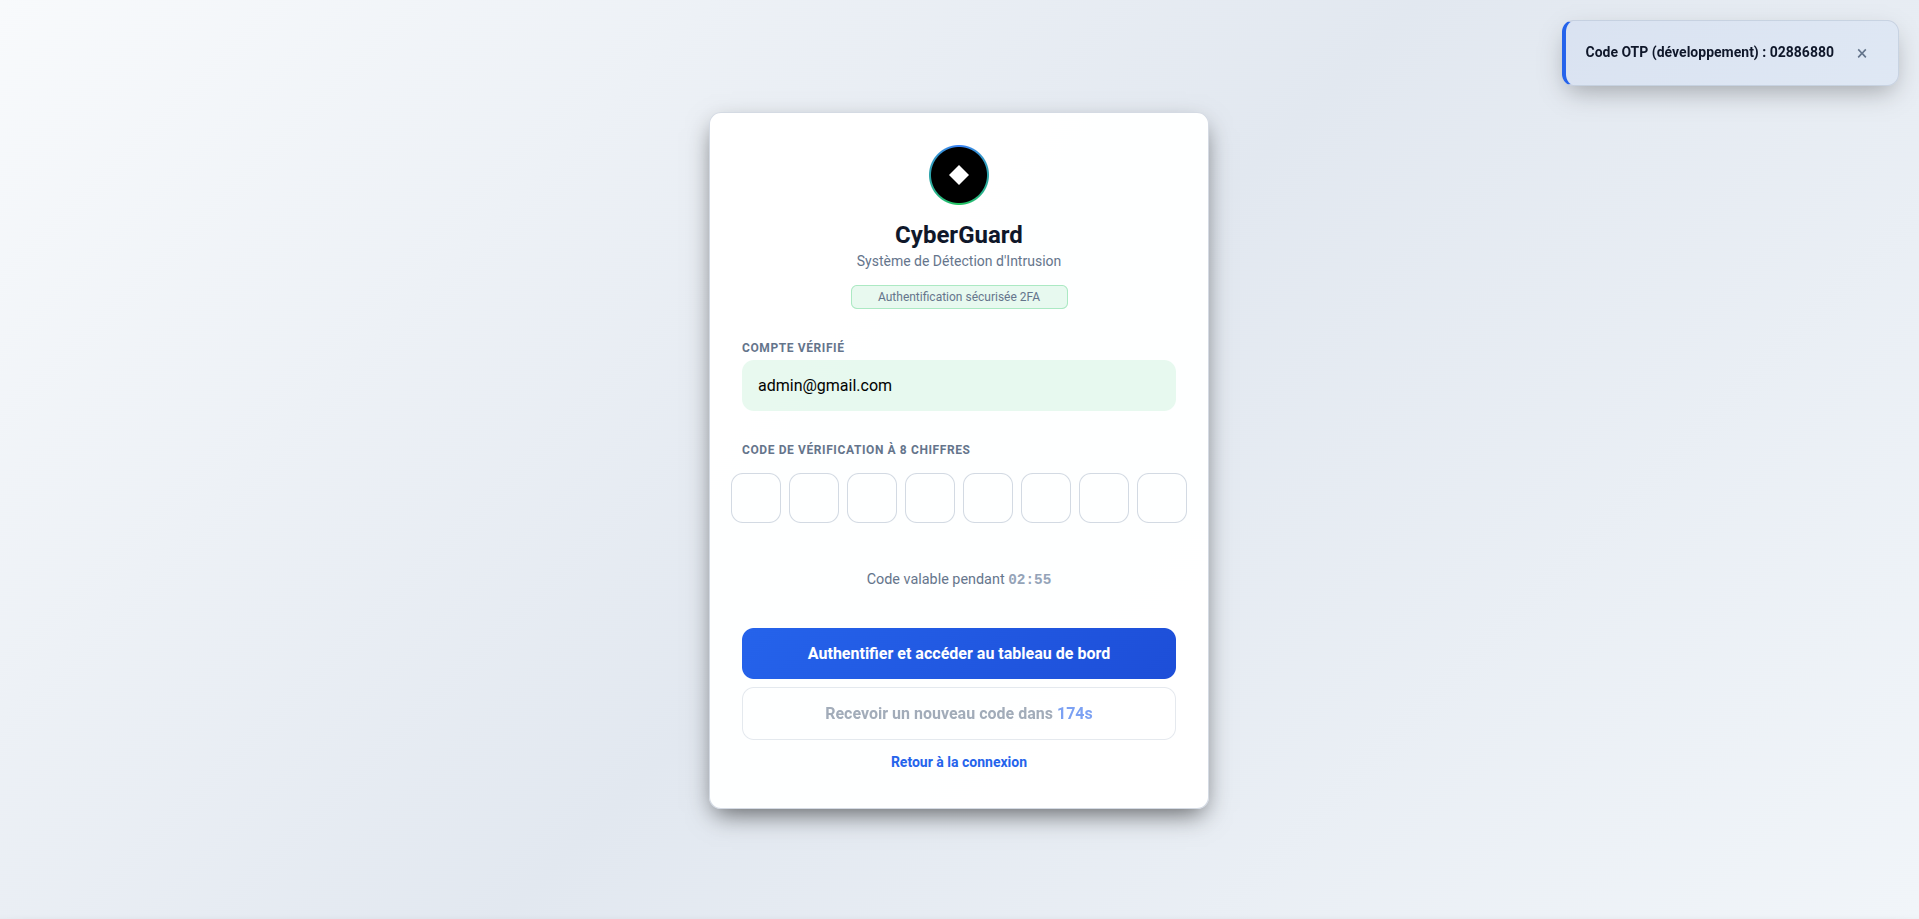
\includegraphics[width=0.8\textwidth]{images/vue-login-OTP.png}
        \caption{Vue connexion email + OTP - CyberGuard}
    \end{figure}
    
    \subsection{Tableau de bord de supervision}
    
    \begin{figure}[H]
        \centering
        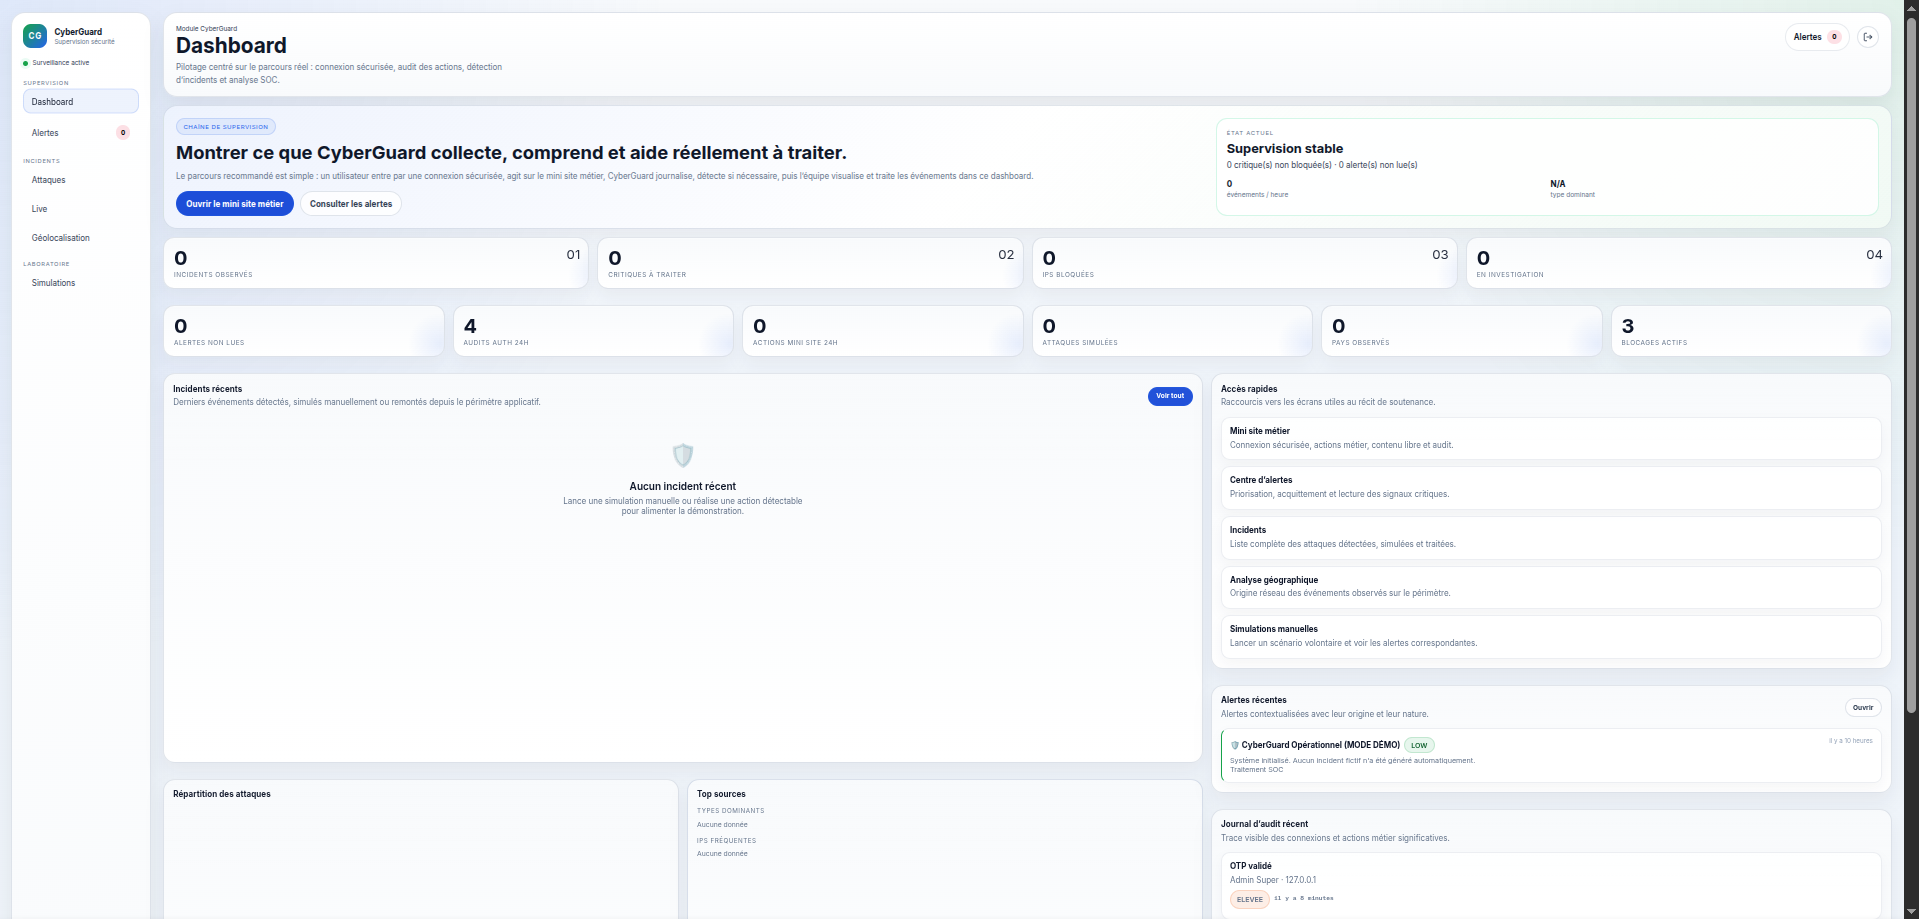
\includegraphics[width=0.8\textwidth]{images/vue-admin-dashboard.png}
        \caption{Vue tableau de bord de supervision - CyberGuard}
    \end{figure}
    
    \subsection{Centre d'alertes}
    
    \begin{figure}[H]
        \centering
        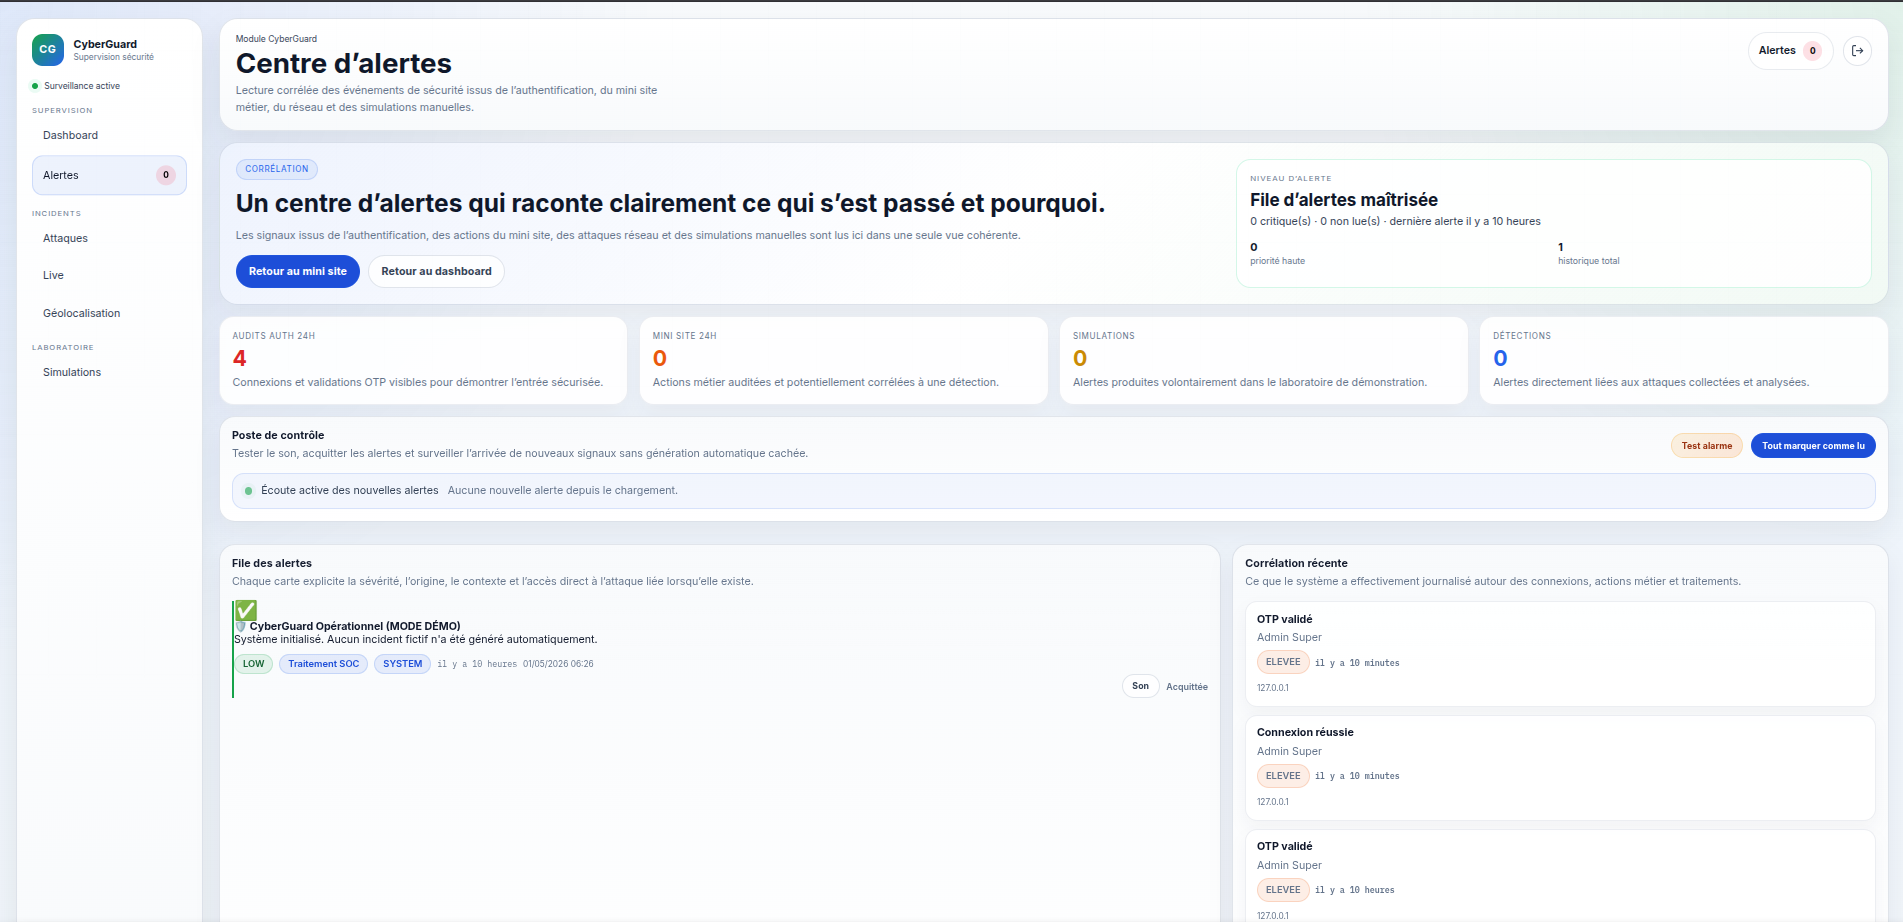
\includegraphics[width=0.8\textwidth]{images/vue-admin-alert.png}
        \caption{Vue centre d'alertes - CyberGuard}
    \end{figure}
    
    \subsection{Gestion des incidents}
    
    \begin{figure}[H]
        \centering
        
\includegraphics[width=0.8\textwidth]{images/vue-admin-incidents.png}
        \caption{Vue gestion incidents - CyberGuard}
    \end{figure}
    
    \subsection{Mini Site métier}
    
    \begin{figure}[H]
        \centering
        
\includegraphics[width=0.8\textwidth]{images/vue-mini-site.png}
        \caption{Vue mini site - CyberGuard}
    \end{figure}
    
    \begin{figure}[H]
        \centering
        
\includegraphics[width=0.8\textwidth]{images/vue-mini-site-usagers.png}
        \caption{Vue mini site usagers - CyberGuard}
    \end{figure}
    
    \begin{figure}[H]
        \centering
        
\includegraphics[width=0.8\textwidth]{images/vue-mini-site-services.png}
        \caption{Vue mini site services - CyberGuard}
    \end{figure}
    
    \begin{figure}[H]
        \centering
        
\includegraphics[width=0.8\textwidth]{images/vue-mini-site-messages.png}
        \caption{Vue mini site messages - CyberGuard}
    \end{figure}
    
    \section{Discussion des résultats}
    
    Les résultats obtenus à l’issue du développement du système CyberGuard permettent de mettre en évidence plusieurs éléments importants, tant sur le plan fonctionnel que technique.\\
    
    Sur le plan fonctionnel, le système répond globalement aux objectifs définis dans le cahier des charges. Les principales fonctionnalités, notamment l’authentification sécurisée, la gestion du mini site métier, la détection d’attaques et la supervision via le tableau de bord, ont été correctement implémentées et testées. Le parcours utilisateur est cohérent et permet de démontrer clairement les différentes capacités du système.\\
    
    L’authentification à deux facteurs (mot de passe + OTP) constitue un point fort du système. Elle permet de renforcer significativement la sécurité d’accès et de limiter les risques de compromission des comptes. Les tests effectués montrent que le processus est fiable, tout en restant compréhensible pour l’utilisateur \cite{nist}.\\
    
    Le moteur de détection, volontairement limité à trois types d’attaques (Brute Force, SQL Injection et XSS), s’est révélé efficace dans le cadre de la démonstration. Ce choix de limitation permet d’éviter la complexité excessive et de proposer un système plus lisible et mieux maîtrisé. Les alertes générées sont pertinentes et permettent une analyse claire des incidents via le tableau de bord.\\
    
    L’intégration du mini site métier constitue également un apport important. Elle permet de contextualiser les actions utilisateurs et de produire des données exploitables pour la détection. Ce choix renforce le réalisme du système et facilite sa compréhension lors de la démonstration.\\
    
    Sur le plan technique, l’utilisation du framework Laravel a permis de structurer le projet de manière modulaire et maintenable. La séparation entre les différentes couches (contrôleurs, services, modèles, middlewares) améliore la lisibilité du code et facilite les évolutions futures. Les mécanismes de sécurité intégrés, tels que la gestion des sessions, la protection CSRF et la journalisation, contribuent à la robustesse globale du système \cite{laravel}.\\
    
    Cependant, certaines limites peuvent être relevées. Le système de détection reste volontairement restreint et pourrait être enrichi avec d’autres types d’attaques ou des mécanismes d’analyse plus avancés. De même, certaines fonctionnalités pourraient être optimisées, notamment en termes de performance ou d’ergonomie de l’interface utilisateur.\\
    
    Enfin, bien que le système soit adapté à une démonstration académique, une mise en production réelle nécessiterait des améliorations supplémentaires, notamment en matière de sécurité.
    
    \section{Conclusion}
    
    Ce chapitre a permis de présenter les résultats obtenus suite à la réalisation du système CyberGuard. Les différentes fonctionnalités implémentées ont été validées à travers des tests, démontrant ainsi la cohérence et la fiabilité du système.
    
    Les résultats confirment que les objectifs fixés ont été atteints, tout en mettant en évidence les perspectives d’amélioration possibles. Le système constitue ainsi une base solide pour une évolution future vers une solution plus complète en cybersécurité.
    
    \chapter{CONCLUSION GÉNÉRALE}
    
    Le présent travail avait pour objectif de concevoir et de développer une plateforme de démonstration en cybersécurité, capable de combiner des mécanismes de protection, de détection et de supervision au sein d’une même application. À travers le projet CyberGuard, il a été possible de mettre en œuvre ces différents aspects dans un système cohérent et fonctionnel.
    
    Dans un premier temps, une analyse des besoins a permis d’identifier les principales fonctionnalités attendues, notamment l’authentification sécurisée, la journalisation des actions, la détection d’attaques et la supervision des incidents. Ces éléments ont servi de base à la définition du cahier des charges et à l’orientation des choix techniques.
    
    La phase de conception a permis de structurer le système à travers une architecture modulaire et des diagrammes UML facilitant la compréhension globale du fonctionnement. Une attention particulière a été accordée aux aspects de sécurité, avec l’intégration de mécanismes tels que l’authentification à deux facteurs, la gestion des sessions sécurisées et la limitation des tentatives d’accès.
    
    La phase de réalisation a conduit à la mise en place d’un système opérationnel intégrant un mini site métier servant de support aux scénarios de démonstration. Le moteur de détection, centré sur trois types d’attaques (Brute Force, SQL Injection et XSS), permet de produire des alertes exploitables et de simuler des incidents de sécurité dans un environnement contrôlé.
    
    Les résultats obtenus montrent que le système répond globalement aux objectifs fixés. Il offre une solution fonctionnelle, structurée et adaptée à une démonstration pédagogique en cybersécurité. Toutefois, certaines améliorations restent envisageables, notamment l’extension du système de détection, l’optimisation des performances et le renforcement de certains mécanismes de sécurité pour une utilisation en environnement réel.
    
    En perspective, ce travail pourrait être enrichi par l’intégration de nouvelles techniques de détection basées sur l’intelligence artificielle, l’ajout de scénarios d’attaque plus avancés ou encore le déploiement du système dans un environnement distribué.
    
    En définitive, le projet CyberGuard constitue une contribution intéressante dans le domaine de la sécurité applicative, en illustrant de manière concrète les enjeux liés à la protection, à la surveillance et à la réaction face aux menaces informatiques.
    
    \newpage
    \addcontentsline{toc}{chapter}{Bibliographie}
    \begin{thebibliography}{9}
        
        \bibitem{owasp}
        OWASP Foundation, OWASP Top 10, \url{https://owasp.org}
        
        \bibitem{nist}
        NIST, Digital Identity Guidelines, \url{https://nist.gov}
        
        \bibitem{iso27001}
        ISO/IEC 27001 Standard
        
        \bibitem{ibm_siem}
        IBM Security, SIEM Overview
        
        \bibitem{ids}
        Intrusion Detection Systems - Concepts and Techniques
        
        \bibitem{qradar}
        IBM QRadar Documentation
        
        \bibitem{elk}
        Elastic Stack Documentation
        
        \bibitem{laravel}
        Laravel Documentation, \url{https://laravel.com}
        
    \end{thebibliography}
    
\end{document}
